\section{Review of the calibration problem and methods}
In this section we will summarize \cite{guo2017calibration}'s findings and propositions on the topic of neural network calibration.

\subsection{The general problem of neural network model calibration degradation}
\cite{guo2017calibration} discovered that they could not confirm \cite{niculescu2005predicting}'s observation that neural networks (for binary classification) were typically well-calibrated for the latest generation of deep neural network models. \cite{lecun1998gradient}'s 5-layer LeNet was compared to \cite{he2016deep}'s 110 layer ResNet on the CIFAR-100 dataset. This comparison is visualized in figure \ref{fig:lenet_vs_resnet_calibration_guo_et_al}, where the top row shows prediction confidence histograms and the bottom row shows reliability diagrams (RDs). RDs show a model's accuracy as a function of its confidence. A perfectly callibrated model has a 45° angled line as its RD. Figure \ref{fig:lenet_vs_resnet_calibration_guo_et_al} shows a striking overconfidence of the ResNet on CIFAR-100 while showing the LeNet has an almost perfect RD on it. \cite{guo2017calibration} thus proposes that the modern ResNet has gained in accuracy over the older LeNet by, through some mechanism, sacrificing calibration. Through abductive reasoning \cite{guo2017calibration} hypothesizes and substantiates that this is a general and explainable evolutionary trend in artificial neural network R\&D that one could call calibration degradation. 

\begin{figure}[htbp!]
  \centering
  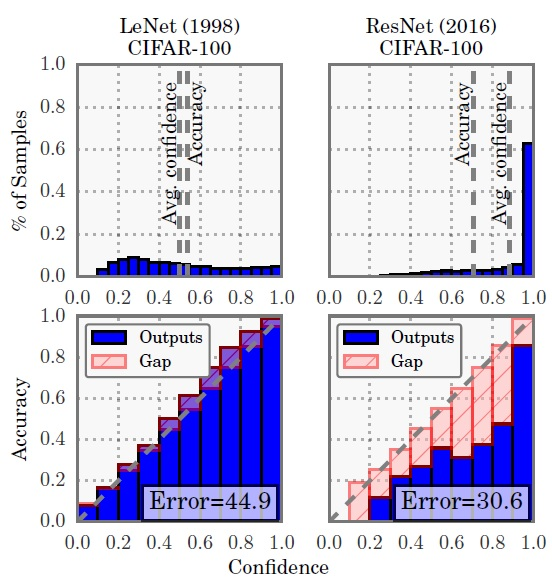
\includegraphics[width=0.6\linewidth]{images/lenet_vs_resnet_calibration_guo_et_al.jpg}
  \caption[5-layer LeNet's vs. 110-layer ResNet's calibration.]{5-layer LeNet (left) vs. 110-layer ResNet (right) calibration.}
  \label{fig:lenet_vs_resnet_calibration_guo_et_al}
  \source{\cite{guo2017calibration}}
\end{figure}
\newpage

%...
%This formula $f(x) = x^2$ is an example.
%...

\subsection{Calibration metrics}
\cite{guo2017calibration} enumerate several calibration metrics for supervised multiclass classification.

\subsubsection{Supporting definitions and notation}
The input $X \in \mathcal{X}$ and label $Y \in \mathcal{Y}=\{1, \ldots, K\}$ are random variables that follow a ground truth joint distribution $\pi(X, Y)=$ $\pi(Y \mid X) \pi(X)$. Let $h$ be a neural network with $h(X)=$ $(\hat{Y}, \hat{P})$, where $\hat{Y}$ is a class prediction and $\hat{P}$ is its confidence or self-estimated probability of correctness. $\hat{P}$ should be calibrated, i.e. represent a true probability. Formally, perfect calibration is defined as $$\mathbb{P}(\hat{Y}=Y \mid \hat{P}=p)=p, \quad \forall p \in[0,1]$$

% where the probability is over the joint distribution. Achieving perfect calibration is impossible in practice. Additionally, the probability in (1) cannot be computed using finitely many samples since $\hat{P}$ is a continuous random variable. This motivates the need for empirical approximations that capture the essence of (1).

% Reliability Diagrams (e.g. Figure 1 bottom) are a visual representation of model calibration (DeGroot \& Fienberg, 1983; Niculescu-Mizil \& Caruana, 2005). These diagrams plot expected sample accuracy as a function of confidence. If the model is perfectly calibrated - i.e. if (1) holds - then the diagram should plot the identity function. Any deviation from a perfect diagonal represents miscalibration

% To estimate the expected accuracy from finite samples, we group predictions into $M$ interval bins (each of size $1 / M$ ) and calculate the accuracy of each bin. Let $B_{m}$ be the set of indices of samples whose prediction confidence falls into the interval $I_{m}=\left(\frac{m-1}{M}, \frac{m}{M}\right] .$ The accuracy of $B_{m}$ is
% $$
% \operatorname{acc}\left(B_{m}\right)=\frac{1}{\left|B_{m}\right|} \sum_{i \in B_{m}} \mathbf{1}\left(\hat{y}_{i}=y_{i}\right)
% $$
% where $\hat{y}_{i}$ and $y_{i}$ are the predicted and true class labels for sample $i$. Basic probability tells us that acc $\left(B_{m}\right)$ is an unbiased and consistent estimator of $\mathbb{P}\left(\hat{Y}=Y \mid \hat{P} \in I_{m}\right)$. We define the average confidence within bin $B_{m}$ as
% $$
% \operatorname{conf}\left(B_{m}\right)=\frac{1}{\left|B_{m}\right|} \sum_{i \in B_{m}} \hat{p}_{i}
% $$
% where $\hat{p}_{i}$ is the confidence for sample $i . \operatorname{acc}\left(B_{m}\right)$ and $\operatorname{conf}\left(B_{m}\right)$ approximate the left-hand and right-hand sides of (1) respectively for bin $B_{m}$. Therefore, a perfectly calibrated model will have $\operatorname{acc}\left(B_{m}\right)=\operatorname{conf}\left(B_{m}\right)$ for all $m \in\{1, \ldots, M\} .$ Note that reliability diagrams do not display the proportion of samples in a given bin, and thus cannot be used to estimate how many samples are calibrated.







\section{Review of applications of interest}
In this work we want to evaluate and analyze the impact of calibration on representative DeepProbLog use-cases where it presents a considerable issue. Unfortunately, these use-cases are not a given. To find and choose some, we first required that:
\begin{itemize}
  \item using PLP with neural predicates to tackle it is appropriate
  \item it is widely studied in neuro-symbolic integration research
  \item there is room to improve it through callibrating (parts of) models
\end{itemize}
If the first and third criterions are not met, there is no reason to use DeepProbLog and/or calibration and the knowledge we'd gain and features we'd create would not necessarily be relevant to our target audience. That's why we disregard most well-known AI toy problems such as playing chess, the N-queens problem and MNIST digit recognition and we start with reservations about using the DeepProbLog demonstration problems showcased by \cite{manhaeve2018deepproblog}. But we do require widely used challenges like the general AI toy problems so that our work's properties and performance can be easily compared to those of other approaches (\cite{russell2002artificial}), hence our second criterion. \par
We then performed a shallow literature scan of neuro-symbolic integration to find recurring themes and toy problems in this field of research. The scientific literature search engines Google Scholar (by Google) and Limo (by KU Leuven) were used to search for papers containing the keywords "neuro", "symbolic" and "integration" simultaneously. 63 random papers were chosen from the results. A breakdown of the problem categories these papers work in is given in table \ref{subject_breakdown}. Papers can work in multiple categories, the count column shows how many work in the category and the \% column shows what percentage of the 63 work in it.
\begin{table}[!htbp]
\centering
\begin{tabular}{ |c|c|c| }
 \hline
 \textbf{Category} & \textbf{Count} & \textbf{\%} \\
 \hline
 Acoustic information processing & 1 & 1.59\% \\
 \hline
 Actuarial science & 2 & 3.17\% \\
 \hline
 Natural sciences modelling & 2 & 3.17\% \\
 \hline
 Control theory & 4 & 6.35\% \\
 \hline
 Fraud detection & 1 & 1.59\% \\
 \hline
 Natural language processing & 7 & 11.11\% \\
 \hline
 Numerical analysis & 1 & 1.59\% \\
 \hline
 Robotics & 2 & 3.17\% \\
 \hline
 Social \& political sciences & 2 & 3.17\% \\
 \hline
 Symbolic knowledge \& structured data processing & 33 & 52.38\%  \\
 \hline
 Visual information processing & 16 & 25.40\%  \\
 \hline
\end{tabular}
\caption{Subfield breakdown of neuro-symbolic integration research}
\label{subject_breakdown}
\end{table}